\section*{Условия}
\subsection*{Задача 1}
	Учитель дал квадратное уравнение вида $x^2 + bx + c$, где $b < 100$ и корни являются натуральным числами большими 1. Затем он сообщил Васе коэффициент $b$, а Пете коэффициент $c$ и попросил их угадать корни, после чего последовал диалог:\\
	Петя: ``Я не знаю корни''\\
	Вася: ``Я знаю, что ты не знаешь''\\
	Петя: ``Теперь я знаю корни''\\
	Вася: ``И я тоже теперь их знаю''\\
	Определите корни данного уравнения.
\vskip 0.4in

\subsection*{Задача 2}
	Игорь взял колоду из 36 карт, после чего загадал одну и сказал Васе масть, а Пете достоинство, после чего выложил на стол следующие карты:\\
	\begin{figure}[!h]
		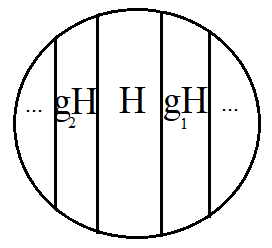
\includegraphics[width=0.9\linewidth]{Pic1}
	\end{figure}
	\vskip 0.1in
	И попросил угудать загаданную, после чего произошел следующий диалог:\\
	Вася: ``Я не знаю какую карту загадал Игорь, но знаю, что и ты тоже не знаешь''\\
	Петя: ``Изначально я не знал какую карту загадал Игорь, но теперь знаю''\\
	Вася: ``И я теперь тоже знаю''\\
	Какую карту загадал Игорь?
\vskip 0.4in

\subsection*{Задача 3}
	Рассмотрим остров с 100 зеленоглазых, заметим что при добавлении людей с другим цветом глаз(без ограничения общности - кареглазых) или замене $100$ человек на $n$ решение не меняется. Предположим что на острове могут встречаться различные цвета глаз, мудрец сказал обитателям о наличии хотя бы $1$ зеленоглазого, а также на острове есть ровно $1$ слепой. Как будет развиваться ситуация и кто сможет покинуть остров, если жители отвечают (а) поочередно, (б) одновременно?

\newpage
\section*{Решения}
\subsection*{Задача 1}
	Заметим, что так как Петя изначально сказал что он не знает корни, то $c$ не является произведением 2 простых (иначе бы он однозначно определил корни), а Петино число раскладывается на $\geqslant 3$ простых, причем не является 3 степенью какого-либо числа. Тогда можно заметить, что так как Вася сказал, что он знает, что Петя не знает корни, то $b$ нельзя представить в виде суммы 2 простых, иначе бы Вася не был уверен в том, что Петя не знает корни. Так как Петя сказал что он знает корни, то его число можно не более чем одним способом разложить на 2 множителя так, чтобы сумма этих множителей была непредставима в виде суммы двух простых. Отбрасывая варианты таким образом можно понять, что $b = 17$, а $c = 52 = 2^2 \cdot 13$, откуда следует что корни это $4, 13$. 
\vskip 0.4in

\subsection*{Задача 2}
	Так как Вася сказал, что он не знает карту и Игорь не знает карту, то масть точно не червы(так как среди них есть валет, которого больше нигде нет, а соостветственно Вася бы не мог утверждать что Петя не знает карту, если бы это были червы) и не бубны(так как среди них есть $9$, которой больше нигде нет). Далее Петя говорит что изначально не знал какую карту загадал Игорь, но из высказывания Васи он сделал вывод, что масть либо пики, либо трефы, тогда карта не дама и не туз, так как полученной из фразы Васи информации было бы недостаточно для того, чтобы отличить пиковую карту от треф, а следовательно это либо 6 трефы, либо 8 пики, либо 10 трефы. Так как После этого вася сказал что тоже теперь знает карту, то это 8 пики, так как если бы масть была трефы, то он бы не смог отличить 6 от 10.
\vskip 0.4in

\subsection*{Задача 3}
	(а) Если у слепого глаза не зеленые, то задача не изменилась и все $k$ зеленоглазых покинут остров на $k$ день. Если у слепого глаза зеленые то он скажет об этом на $n$ день, так как будет знать, что если у него глаза не зеленые, то он услышет что у кого-то зеленые глаза до $n$ дня. При этом никто больше не покинет остров так как будет известно, что 1 зеленоглазый его покинул, а следовательно оставшиеся обитатели уже не смогут руководствоваться указанием по поводу хотя бы 1 зеленоглазого. 
	\vskip 0.1in
	(б) Рассмотрим сперва задачу без слепого, заметим что если обитатели острова поочердено говорят о знании/незнании цвета своих глаз, то в первый день последний говоряий зеленоглазый скажет что знает цвет всех глаз, так как будет знать что все остальные зеленоглазые не знают свой цвет. Соответственно все говорящие после него в этот же день будут знать что их цвет глаз не зеленый. Больше никто не покинет остров так как все будут видеть что зеленоглазый его покинул, а следовательно информация о хотя бы 1 зеленоглазом на остров будет устаревшей.\\
	Теперь добавим слепого, если кто-то до него сказал что знает свой цвет глаз(зеленый), то задача не изменилась. Если слепой говорит самым последним и никто до него не сказал про зеленый цвет глаз, то слепой говорит что у него зеленый цвет глаз и никто больше не покидает остров. Если же слепой не последний и до него никто не сказал по зеленый цвет глаз, то он тоже не может это сказать, так как у него может быть какой-то другой цвет, а последний зеленоглазый говорит после него, тогда на следующий день, если никто так и не скажет про зеленый цвет глаз, слепой узнает о том, что его цвет глаз зеленый(так как хотя бы 1 зеленый все еще есть и никто не сказал что у него зеленый цвет), если же кто-то в первый день сказал что у него зеленый цвет глаз, то слепой так и не покинет остров, как и все зеленоглазые оставшиеся на нем после первого дня.
	\vskip 0.4in


	(*)Также можно рассмотреть задачу о том, что следует говорить мудрецу, чтобы спасти максимальное число людей в обоих случаях, если среди людей есть (а) $m$ слепых, их распределение по цветам глаз неизвестно, (б) $m$ слепых, их распределение по цветам глаз известно.